\emph{Deep Learning} (DL), também conhecido como Aprendizagem Profunda, compreende um conjunto de técnicas de ML que podem ser aplicadas em problemas de aprendizado supervisionado e não-supervisionado. A principal característica dos modelos neste domínio é a capacidade de representar e reconhecer características complexas, por meio da adição de níveis ou camadas de operações não lineares, como nas redes neurais profundas, máquinas de Boltzmann profundas e fórmulas proposicionais. Modelos deste tipo ganharam popularidade ao se mostraram capazes de resolver problemas complexos com uma acurácia cada vez maior \cite{bengio2009learning}.

O bom desempenho de modelos de DL é decorrente do aumento recente da quantidade de dados disponíveis sobre temas complexos, aliado com o aumento da disponibilidade de recursos computacionais para executar modelos mais robustos \cite{goodfellow2016deep}. Atualmente, segundo a IBM, são gerados $2,5$ quintilhões de bytes de dados por dia, e 90\% do volume de dados presente no mundo hoje foi criado nos últimos dois anos \cite{ibm2017bigdata}.

\subsubsection{Breve Histórico}

Historicamente, o conceito de deep learning se originou de pesquisas sobre Redes Neurais Artificiais (RNA). A história da pesquisa sobre este modelo está dividida em três ondas, ou gerações. A primeira geração foi marcada pelo desenvolvimento dos modelos Perceptron e Adaline, além do algoritmo de Backpropagation. A segunda onda?. A teceira onda começa em 2006 com a publicação do artigo -- sobre redes de crença profunda.

Os avanços recentes alcançados no campo da visão computacional foram atingidos utilizando modelos de redes neurais convolucionais com várias camadas.


\subsection{Redes Neurais Convolucionais Profundas}
Redes neurais convolucionais (CNN, do inglês, \emph{Convolutional Neural Networks}) são uma classe de redes neurais \emph{feed-forward} profundas que têm se mostrado bem-sucedidas na análise de imagens.

específico para o processamento de dados que têm uma topologia bem definida e estruturada em uma grade, a exemplo de séries temporais e imagens. Sua principal característica envolve o uso de convoluções no lugar de multiplicações de matrizes em ao menos uma das camadas da rede neural\cite{goodfellow2016deep}. Este modelo pode ser aplicado em tarefas de classificação, regresssão, localização, detecção, entre outros.

\todo{Precisa também refatorar mais o texto para permitir revisão.}

Cada camada das redes neurais convolucionais é composta por uma etapa de convolução, seguida por uma ativação não-linear, finalizando em \emph{pooling}, como mostra a Figura \ref{fig:cnn_camada}. A seguir, serão explanadas cada uma destas etapas. \todo{Figura em português, please. Usar o software Ipe para desenhar. Incluir na legenda. Fonte: \ldots}

\begin{figure}
	\centering
	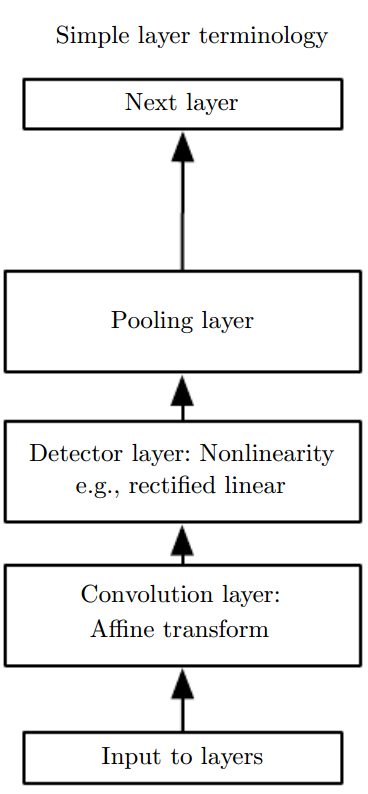
\includegraphics[height=0.5\textheight]{img/cnn_camada.png}
	\caption{Componentes de uma camada de uma rede neural convolucional \cite{goodfellow2016deep}. }
	\label{fig:cnn_camada}
\end{figure}


\subsubsection{Convolução}
A operação de convolução descreve a média ponderada de uma determinada função $x_1(t)$ sob um intervalo fixo de uma variável, enquanto os pesos da média ponderada considerada pertencem à função $x_2(t)$ amostrados em intervalos $a$ \cite{bracewell1986fourier}. Assim, a convolução $s(t)$ de duas funções $x_1(t)$ e $x_2(t)$ é uma função $f: \mathds{Z} \rightarrow \mathds{R}$ representada simbolicamente por $x_1(t) * x_2(t)$ e definida de acordo com a Equação \ref{eq:int_convolucao} \cite{lathi2006sinais}.
\begin{equation}\label{eq:int_convolucao}
	s(t) = x_1(t) * x_2(t) = \int_{-\infty}^{\infty} x_1(a) x_2(t-a)da
\end{equation}

Quando a operação de convolução é aplicada em aprendizagem de máquina, a primeira função $x_1(t)$ é chamada de \emph{input (entrada?)}, a segunda função $x_2(t)$ é chamada de \emph{kernel (núcleo?)}, e a saída $s(t)$ é chamada de mapa de \emph{feature map (mapa de características?)}. Neste caso, a entrada normalmente é um vetor multidimensional de dados e o núcleo é um vetor multidimensional de pesos que devem ser adaptados pelo algoritmo de aprendizado de máquina. Em redes neurais convolucionais, os vetores multidimensionais de entrada e núcleo são chamados tensores. Além disto, assume-se que os valores dos tensores são zero em todos os pontos menos os que estão guardados em memória, ou seja, a operação de convolução é implementada apenas nas posições declaradas dos vetores de dados e peso. Assim, para uma imagem bidimensional de tamanho $(m,n)$ $I$ como entrada, tem-se um núcleo bidimensional $K$, e a operação de convolução é definida como exemplificado na Equação \ref{eq:conv_img}, para cada posição $(i,j)$ do mapa de características resultante \cite{goodfellow2016deep}.

\begin{equation}\label{eq:conv_img}
	S(i,j) = I(i,j)*K(i,j) = \sum_{m}\sum_{n}I(m,n)K(i-m,j-n)
\end{equation}

A convolução é comutativa, ou seja, as Equações \ref{eq:conv_img_eq} e \ref{eq:conv_img} são equivalentes, salvo que no primeiro caso há a convolução da imagem pelo núcleo, enquanto no segundo há a convolução do núcleo pela imagem. Comumente, a Equação \ref{eq:conv_img} é a implementada em algoritmos de redes neurais convolucionais, haja visto que existem menor variação no intervalo de valores válidos de $m$ e $n$, o que diminui o custo computacional.

\begin{equation}\label{eq:conv_img_eq}
	S(i,j) = K(i,j)*I(i,j) = \sum_{m}\sum_{n}I(i-m,j-n)K(m,n)
\end{equation}

A propriedade comutativa surge graças à ação de revolver o núcleo em relação à imagem, e não tem aplicação prática. Porém, esta propriedade não tem fins práticos além da prova da operação de convolução. Assim, é comum que seja implementada correlação cruzada, indicada na Equação \ref{eq:correlacao_img_eq}, semelhante à convolução dada na Equação \ref{eq:conv_img_eq} sem que haja o espelhamento do núcleo em relação à imagem.

\begin{equation}\label{eq:correlacao_img_eq}
	S(i,j) = I(i,j)*K(i,j) = \sum_{m}\sum_{n}I(i+m,j+n)K(m,n)
\end{equation}

\subsubsection{Ativação}


\subsubsection{Pooling}

Depois de realizar várias operações de convolução em paralelo para gerar um conjunto de ativações lineares e alimentá-las a funções de ativação não-lineares, como \emph{ReLU}, \emph{Softmax}, etc, na chamada etapa de detecção, chega-se à etapa de \emph{pooling}. Uma função de \emph{pooling} substitui a saída da rede em determinada localização por uma síntese estatística das saídas vizinhas. Por exemplo, a função \emph{max pooling} retorna o valor máximo em uma área retangular, enquanto a \emph{average pooling} retorna a média das saídas de um retângulo. %O objetivo destas funções é fazer com que
